\errorcontextlines=10
\documentclass[12pt]{report}
\usepackage[a4paper, left=2cm, right=2cm, top=2cm, bottom=2cm]{geometry}
\usepackage[utf8]{inputenc}
\usepackage[T1]{fontenc}
\usepackage{graphicx}
\usepackage[french]{babel}
\usepackage[backend=biber,style=numeric]{biblatex}
\usepackage[acronym]{glossaries}
\usepackage[hidelinks]{hyperref}
\usepackage[anythingbreaks]{breakurl}

\title{Des échecs de l'informatique}
\author{Nicolas Sentout \\ Maxime Pacaud \\ Lorian Corbel}

\addbibresource{biblio.bib}
\makeglossaries

\parskip=5pt plus2pt minus 1pt
\frenchbsetup{ReduceListSpacing=false}

\begin{document}

% ACRONYM
\newacronym{IP}{IP}{Internet Protocol}
\newacronym{TCP}{TCP}{Transport Control Protocol}
\newacronym{OSI}{OSI}{Open Systems Interconnection}
\newacronym{PTT}{PTT}{Postes, Télégraphes et Téléphones}
\newacronym{DGT}{DGT}{Direction Générale des Télécommunications}
\newacronym{CNET}{CNET}{Centre National d'Études des Télécommunications}
\newacronym{ETCD}{ETCD}{Équipement de Terminaison de Circuit de Données}
\newacronym{ETTD}{ETTD}{Équipement Terminal de Traitement de Données}
\newacronym{DARPA}{DARPA}{Defense Advanced Research Projects Agency}
\newacronym{INRIA}{INRIA}{Institut National de Recherche en Informatique et en Automatique}
\newacronym{CCITT}{CCITT}{Comité Consultatif International Télégraphique et Téléphonique}
\newacronym{ARPANET}{ARPANET}{Advanced Research Projects Agency Network}
\newacronym{CNES}{CNES}{Centre National d'Études Spatiales}
\newacronym{CVP}{CVP}{Circuit Virtuel Permanent}
\newacronym{CVC}{CVC}{Circuit Virtuel Commuté}
\newacronym{ESA}{ESA}{European Space Agency}
\newacronym{EAL}{EAL}{Evaluation Assurance Level}
\maketitle
\tableofcontents

% ~=~=~=~=~=~=~
% ERP FOX MEYER
% ~=~=~=~=~=~=~
\chapter{L'échec de l'ERP de FoxMeyer}

\section{Qu'est-ce qu'un ERP ?}

Un logiciel \textbf{ERP} (Enterprise Resource Planning ou PGI pour Progiciel de Gestion Intégré en français) est un outil informatisé qui permet le pilotage de l’entreprise. Sa particularité est d’embarquer, en un même logiciel et une seule base de données, les fonctionnalités nécessaires à la gestion de l’ensemble de l’activité d’une entreprise : gestion comptable, gestion commerciale, gestion des stocks…

Selon la définition donnée par le CXP, le premier cabinet européen d’analyse et de conseil dans le domaine des logiciels, un ERP doit :
\begin{itemize}
\item émaner d'un concepteur unique
\item garantir à l'utilisateur l'unicité d'information assurée par la disponibilité de l'intégralité de la structure de la base de données à partir de chacun des modules, même pris individuellement
\item reposer sur une mise à jour en temps réel des informations modifiées dans tous les modules affectés
\item fournir des pistes d'audit basées sur la garantie d'une totale traçabilité des opérations de gestion
\item couvrir soit une fonction (ou filière) de gestion, soit la totalité du système d'information de l'entreprise\cite{divaltoerp}.
\end{itemize}

\section{Le contexte de l'échec}

Au début des années 90, \textit{FoxMeyer}, une entreprise dans le domaine de la santé, était le 4ème plus grand distributeur pharmaceutique aux États-Unis, avec un chiffre d’affaires de 5 milliards de dollars et plus de 500 000 produits distribués quotidiennement\cite{exoplatfoxmeyer}. Elle avait à ce moment-là pour but d’utiliser la technologie pour augmenter son efficacité. Ainsi débuta le projet Delta III en 1993.
\textit{FoxMeyer} conduit une étude de marché et une évaluation de produits et acheta SAP R/3, un ERP développé par l’entreprise allemande \textit{SAP}, cette même année.
Elle acheta également un système d’automatisation d’entrepôt d’un vendeur appelé \textit{Pinnacle} et choisit \textit{Andersen Consulting} pour intégrer et mettre en place les 2 systèmes. La réalisation du projet Delta III se fera en 1994 et 1995.

Selon le président directeur général de \textit{Pinnacle}, l’échec du projet n’était pas un problème d’automatisation ni un problème logiciel mais un échec de gestion de projet.
\textit{FoxMeyer} a fait faillite en 1996 et annonça en 1998 qu’elle poursuivait en justice \textit{SAP} ainsi que \textit{Andersen Consulting} pour 500 millions de dollars chacun\cite{zimmerfoxmeyer}.

\section{Le problème plus en détail}

La mise en place de ce projet de plusieurs millions de dollars était le premier du genre dans l’industrie pharmaceutique. L’implémentation de SAP R/3 aura coûté à \textit{FoxMeyer} 100 millions de dollars alors que l’entreprise espérait pouvoir faire à l’aide de cet ERP 40 millions de dollars d’économie par an.

Suite à l’échec de ce projet, une mauvaise organisation du projet dès la phase de cahier des charges jusqu’au aux étapes d’implémentations a été mise en avant\cite{zimmerfoxmeyer}.
Il y a tout d’abord eu plusieurs erreurs au niveau de la planification. \textit{FoxMeyer} a choisi un ERP non compatible avec son activité. En effet, après plusieurs tests, il s’est avéré que le SAP R/3 ne pouvait traiter que 10 000 commandes par nuit comparé à 420 000 avec l’ancien système qu'utilisait \textit{FoxMeyer}. Un autre problème est que l’entreprise n’a pas écouté l’avis d’autres consultants et a basé son choix uniquement sur la réputation d'\textit{Andersen Consulting} et \textit{SAP}. On notera également qu’aucun plan d’urgence n’avait été mis en place en cas de déroute du projet.

On peut ensuite citer plusieurs problèmes dans la phase d’implémentation :
\begin{itemize}
\item aucune restructuration du processus opérationnel
\item phase de test bâclée
\item une portée du projet beaucoup trop ambitieuse
\item projet beaucoup tourné vers les intérêts des collaborateurs IT
\item mauvais management et peu de support
\item manque de coopération de la part des utilisateurs\cite{zimmerfoxmeyer}.
\end{itemize}

\section{Les solutions possibles}

L'échec de la mise en place de l'ERP est dû à plusieurs problèmes qui auraient pu être évités si \textit{FoxMeyer} avait mieux planifié et gérer son projet. Certaines méthodes et outils de gestion de projet auraient dû être privilégiés.

\subsection{Qu'est-ce que la gestion de projet ?}

La gestion de projet est une démarche visant à organiser de bout en bout le bon déroulement d'un projet.
La norme ISO 9000 décrit un projet comme un « processus unique, qui consiste en un ensemble d'activités coordonnées et maîtrisées comportant une date de début et une date de fin, entrepris dans le but d'atteindre un objectif conforme à des 
exigences spécifiques, incluant des contraintes de délais, de coûts et de ressources »\cite{wikigestion}.

Les acteurs principaux d'un projet sont le maître d'ouvrage (MOA), le maître d’œuvre (MOE) et l'utilisateur.
Le \textbf{maître d'ouvrage} est le représentant du client. A partir des demandes des futurs utilisateurs, il établit un cahier des charges puis passe un contrat avec le fournisseur.
Le \textbf{maître d’œuvre} est celui qui réalise le projet. Dans le cas de \textit{FoxMeyer}, \textit{Andersen Consulting} a été choisi pour implémenter l'ERP.
L'\textbf{utilisateur} apporte l'expression des besoins. Un des problèmes de \textit{FoxMeyer} vient de cet acteur. En effet, il a été reporté que certains utilisateurs n'étaient pas très engagés. C'est compréhensible étant donné que leur travail était menacé par le projet d'automatisation de l'entrepôt\cite{zimmerfoxmeyer}.

Un projet a également 3 contraintes caractéristiques :
\begin{itemize}
\item les objectifs du projet ou sa portée
\item les délais dont on dispose pour finir le projet
\item le coût\cite{wikigestion}.
\end{itemize}

On peut représenter ces 3 contraintes comme ceci sur la figure \ref{fig:trg}.
\begin{figure}[htp]
  \centering
  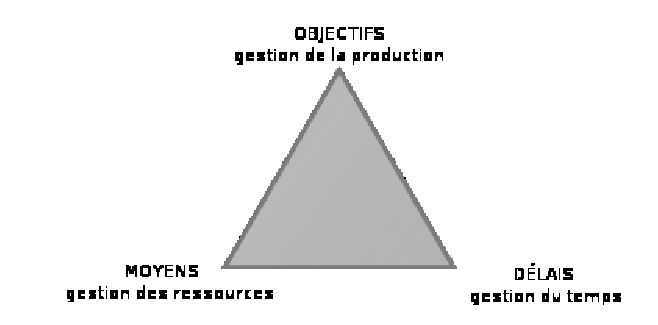
\includegraphics[scale=0.8]{images/triangle_projet}\cite{wikiprojet}
  \caption{Triangle de projet}
  \label{fig:trg}
\end{figure}

Il faut retenir que les 3 côtés sont liés : si l'un est modifié, les autres le seront également.

La gestion de projet s’astreint à ces 3 contraintes pour répondre aux exigences de compétitivité des entreprises et d’adaptation aux évolutions du marché dans un environnement de plus en plus complexe et incertain\cite{coursiut}. Pour cela, il est nécessaire de se conformer à des méthodes de gestion, d'organisation et de management…

\subsection{Les méthodes agiles}

Parmi ces méthodes de gestion de projets informatiques, nous retrouvons les méthodes agiles. Ce sont les méthodes les plus communément utilisées en entreprise de nos jours\cite{coursiut}.
Elles sont plus structurées et plus légères que d'autres méthodes traditionnelles et sont censées donner de l'agilité pour contourner les obstacles et s'adapter aux particularités de chaque projet informatique.
Dans ces méthodes, on remarque notamment que les besoins du client peuvent changer et en particulier se préciser (ce qui est en pratique souvent le cas), une plus forte collaboration entre le MOE et le MOA et des itérations courtes qui permettent de produire un livrable à chaque fois opérationnel\cite{wikiscrum}. De plus, l'oral  est privilégié pour la communication entre les différents acteurs\cite{coursiut}. Le client doit rester partie prenante du projet pendant tout le développement.
La vision du travail est également un élément clé : motivation des développeurs, rythme soutenable, équipes auto-organisées, qualité de l'architecture et simplicité des développements, amélioration continue, etc.

On pourrait résumer l'état d'esprit des méthodes agiles avec 4 valeurs :
\begin{itemize}
\item les individus et leurs interactions plus que les processus et les outils
\item des logiciels opérationnels plus qu'une documentation exhaustive
\item la collaboration avec les clients plus que la négociation contractuelle
\item l'adaptation au changement plus que le suivi d'un plan\cite{gitagile}.
\end{itemize}
On retrouve plusieurs méthodes utilisant les modèles agiles mais l'une d'entre elles est devenu très populaire auprès des équipes de développement informatique : Scrum.

\subsubsection{Scrum}

Scrum est un cadre de travail permettant de répondre à des problèmes complexes et changeants tout en livrant de manière productive et créative des produits de la plus grande valeur possible\cite{gitagile}.~~\\
Nous avons précédemment décrit qu'une gestion de projet classique avait 3 acteurs (MOA, MOE, utilisateur). Scrum définit 3 rôles bien distincts pour mener un projet à terme.

Le propriétaire du produit, ou plus couramment appelé le \textbf{Product Owner} (PO) est le premier de ces rôles. Il est le responsable du client et des utilisateurs. C'est celui qui définit les fonctionnalités, les priorise et collabore avec les autres rôles. Il est exigeant et soutient l'équipe en lui donnant de la reconnaissance\cite{wikienscrum}.

L'\textbf{équipe de réalisation} est responsable de la livraison d'une nouvelle version de l'application à chaque itération. Elle ne comporte pas de rôles prédéfinis et est auto-organisée. Cela signifie que que c'est elle qui choisit comment accomplir son travail sans que ce soit imposé par une personne externe à l'équipe.

Le troisième et dernier rôle est le \textbf{Scrum master} (ou maître de mêlée). Son principal but est de faire en sorte que l'équipe de développement n'ait ni obstacles ni distractions et qu'elle puisse travailler dans de parfaites conditions pour délivrer le produit dans les temps.~~\\
Ce n'est pas un chef de projet classique, on pourrait le qualifier comme un « leader au service de l'équipe ». Il aide l'équipe à déterminer quelles interactions avec l'extérieur lui sont utiles et lesquelles sont freinantes.

Outre ces 3 rôles, Scrum fournit aussi des évènements. Chaque évènement est unique mais ils contribuent tous à empêcher le projet de dériver et à accompagner son avancement.

Le premier évènement est le \textbf{sprint} (ou itération) qui est l'unité de base du développement en Scrum. C'est une période d'une semaine à un mois, au bout de laquelle l'équipe de réalisation délivre un incrément du produit, potentiellement livrable. La durée de ce sprint est fixée en avance et n'est pas censée changer pendant le développement du produit. Durant un sprint on ne peut modifier ni l'objet du sprint, ni la composition de l'équipe. Le propriétaire du produit peut décider d'annuler le sprint à tout moment si l'objet de celui-ci devient obsolète. Dans ce cas, les développements terminés sont revus par le propriétaire du produit, qui peut décider de les accepter ou de les refuser. Les éléments du sprint n'étant pas acceptés sont ré-estimés et remis dans le carnet du produit. Un nouveau sprint peut alors démarrer\cite{wikiscrum}.

Une \textbf{planification de sprint} (ou planning) a lieu à chaque début de sprint. C'est une réunion durant laquelle toute l'équipe Scrum est présente. Le but de cette réunion est de décider de la prochaine itération du produit et de décrire comment l'équipe s'organisera pour délivrer cette itération à temps. Durant celle-ci, les participants discutent de la quantité de travail à fournir pendant ce sprint, définissent les fonctionnalités du carnet de produit qui peuvent être complétées en un sprint et préparent un carnet de sprint qui décrit le travail à accomplir pour chaque fonctionnalité du carnet de produit sélectionnée.

La \textbf{mêlée quotidienne} (ou daily Scrum) intervient tous les jours durant un sprint. C'est une réunion très courte (15 minutes en général), à laquelle n'importe qui peut participer ~~\\ ( bien que seuls les membres de l'équipe de développement communiquent ), qui permet de faire un point sur chaque tâche en cours et sur les difficultés rencontrées par chaque développeur.
Chaque développeur répond alors grossièrement à 3 questions :
\begin{itemize}
\item Qu'est-ce que j'ai fait depuis la dernière mêlée ?
\item Qu'est-ce que j'ai l'intention de faire d'ici la prochaine mêlée ?
\item Qu'est-ce qui me freine ou bloque\cite{wikiscrum} ?
\end{itemize}

La mêlée permet donc de synchroniser l'équipe et d'identifier les éventuels retards pris par l'équipe de développement.

La \textbf{revue du sprint} prend place à la fin d'un sprint et dure en général 4 heures. Son objectif est de valider l'incrément de produit qui a été réalisé pendant le sprint.
L'équipe évoque les fonctionnalités finies et celles en cours de développement. Ensuite, elle présente aux personnes qui participent à la revue les nouvelles fonctionnalités développées au cours du sprint.
A la suite de cette présentation, le product owner décide d'accepter ou refuser les fonctionnalités présentées\cite{wikiscrum}.

Enfin, le dernier évènement est la \textbf{rétrospective du sprint}. Seuls les 3 acteurs Scrum peuvent participer. C'est une réunion, un peu moins longue que la revue du sprint, qui se concentre sur le sprint qui vient de se terminer. Elle permet d'améliorer le processus de développement de l'équipe en mettant les idées de chacun à contribution. Pour cela, l'équipe s'interroge sur ce qui a bien fonctionné, ce qui n'a pas fonctionné et ce qui a mal fonctionné\cite{gitagile}. L'équipe de développement en déduit un plan d'actions d'amélioration qu'elle mettra en place lors de l'itération suivante.

Sur le graphique figure \ref{fig:scrum}, on peut clairement voir l'enchaînement de chaque évènement dans un projet lambda.
\begin{figure}[htp]
  \centering
  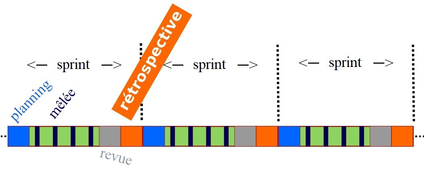
\includegraphics[scale=0.8]{images/events_scrum}\cite{agiscrum}
  \caption{Cycle Scrum}
  \label{fig:scrum}
\end{figure}

Pour finir, les derniers éléments nécessaires au fonctionnement de Scrum sont les artéfacts.

En agilité, on ne produit pas de documentation complète dès le début du projet. On rajoute progressivement des fonctionnalités au produit dans un document appelé le \textbf{carnet de produit} (ou product backlog)\cite{wikiscrum}. Ce carnet contient donc la liste des fonctionnalités attendues du produit, classées selon la quantité de travail demandée. Par exemple, si notre produit est une bibliothèque en ligne, la fonctionnalité « lister tous les livres d'une certaine catégorie » vaudra 1 point et la fonctionnalité « ajouter un livre dans un panier » vaudra 5 points. Le carnet du produit, son évolution et sa publication sont sous la responsabilité du product owner. C'est lui qui décide de changer l'ordre des éléments dans la liste, d'en ajouter, d'en enlever, de modifier leur description, etc. Les éléments en tête de liste sont à prioriser dans le développement et sont mieux décrits et estimés que les autres éléments.

Le \textbf{carnet de sprint} (ou sprint backlog) est le document contenant tout le travail que l'équipe de réalisation doit effectuer pendant le prochain sprint.
Cette liste est construite par l'équipe de développement en sélectionnant des éléments du carnet de produit. L'équipe peut mettre à jour le carnet de sprint à tout moment pendant le sprint afin que celui-ci donne une vision la plus précise possible de ce que l'équipe prévoit de réaliser pour atteindre l'objectif du sprint.

Le dernier artéfact de Scrum est l'\textbf{incrément}. C'est l'ensemble de toutes les fonctionnalités du carnet de sprint qui ont été terminées pendant le dernier sprint plus toutes les fonctionnalités déjà terminées lors des sprints précédents. Les fonctionnalités comprises dans l'incrément doivent être complètes et doivent être telles qu'on pourrait sortir un produit fini fonctionnel intégrant seulement ces fonctionnalités.

% ~=~=~=~=~=~=~=~=~
% Le protocole X.25
% ~=~=~=~=~=~=~=~=~
\chapter{Le protocole X.25}

\section{D'un circuit}

Au début des années 1970, le besoin de définir des protocoles standard afin d'assurer l'interconnexion des réseaux privés à travers les réseaux publics s'est fait ressentir.
À cette époque les protocoles de télécommunications sont par commutation de circuits, qui correspond au branchement matériel de lignes joignant des terminaux. Les informations échangées parcourent toujours le même chemin au sein du réseau durant le temps de la session. Sa simplicité conceptuelle et de mise en œuvre a fait son succès et son emploi dans les premiers réseaux de communication comme le téléphone puis dans les réseaux informatiques balbutiants des années 1950\cite{wikicc}.

En France, la commutation de circuits est mise en avant lorsque la \gls{DGT}, ancêtre de France Télécom, réalise autour de 1970 \og Caducée \fg, un service spécialisé de transmission de données, destiné à répondre à la demande des entreprises en échange de données. Puis c'est le projet Hermès, lancé en 1971, qui vise à intégrer les progrès en commutation électronique. Pour la DGT, c'est un enjeu important face aux réseaux privés, utilisant des liaisons spécialisées. Elle a alors eu besoin de services informatiques pour la programmation ou le calcul, et conserver la gestion des réseaux, afin de ne pas seulement fournir les lignes.

\section{À un paquet}

Malheureusement la commutation de circuits présente un risque de sous-utilisation du support en cas de \og silence \fg pendant la communication.
C'est pour cette raison qu'au même moment, le British Post Office est encouragé à choisir la voie inverse, la commutation de paquets, par le National Physical Laboratory, qui emploie un des pionniers de cette technologie, Donald Davies. La commutation de paquets est fondée sur le découpage des données pour permettre une utilisation rationnelle du réseau. En effet, contrairement à la commutation de circuits les ressources ne sont réservées que durant leur utilisation effective (par exemple: le temps de transfert d'un paquet). Chaque paquet est composé d'un en-tête contenant des informations sur son contenu et sa destination, qui permet au commutateur d'aiguiller le paquet sur le réseau vers son point final\cite{wikicp}.

Le principe de la commutation de paquets, baptisée plus tard \og datagramme \fg, a été imaginé de manière encore abstraite et publié pour la première fois en 1964, et présenté en 1968 à la Conférence d'Edimbourg par Donald Davies, du National Physical Laboratory britannique puis par Paul Baran. Mais en 1971, aucun réseau n'avait encore été conçu de la sorte.

\section{Cyclades}

%(todo : parler du Plan Calcul ? De la CII ?)

C'est l'année durant laquelle une mission d'information technique française, pour le compte du Plan Calcul, effectue un séjour aux États-Unis afin de suivre les tout débuts de l'\gls{ARPANET}, le réseau à transfert de paquets développé aux États-Unis par la \gls{DARPA}. Le projet fut lancé en 1966, mais ARPANET ne vit le jour qu'en 1969. Sa première démonstration officielle date d'octobre 1972\cite{wikiarpa}.

À l'époque, toutes les administrations françaises voulaient mettre en place leurs propres bases de données. Les universités coopèrent au projet par le biais de contrats de recherche et la délégation générale à l'informatique, menée par Maurice Allègre, souhaite les interconnecter via un réseau de données. Michel Monpetit, qui cumule alors les fonctions de principal adjoint de Maurice Allègre au Plan Calcul et de directeur adjoint de l'IRIA, ancêtre de l'\gls{INRIA}, sous la direction du professeur Michel Laudet, recrute Louis Pouzin à l'IRIA pour créer un réseau d'ordinateurs français pour la recherche. Baptisé Cyclades, ce projet public lancé par Maurice Allègre est dirigé par Louis Pouzin. En septembre 1971, il prend la direction de la Délégation à l’Informatique, succédant à Maurice Allègre et se fait héberger par l’IRIA\cite{wikicyc}.

Chargé du projet, Louis Pouzin réunit une petite équipe, qui démarre en 1971 à six personnes environ, et choisit des gens à l’extérieur de l’IRIA comme Jean-Louis Grangé, Jean-Pierre Touchard, Michel Elie, Jean Le Bihan et Gérard Le Lann, qui se rendra chez Arpanet en 1973. Les échanges entre Cyclades et Arpanet, nombreux, ont été facilités par la présence de français dans l'équipe de début d'Arpanet. L'équipe Cyclades entretient des contacts réguliers avec celle qui travaille à Arpanet, notamment avec Vinton Cerf et Bob Kahn.

\section{Les prémices du X.25}

En 1970, Antoine Jousset, du \gls{CNET}, rapporte du \gls{CCITT} des informations sur les projets anglais. Avec Rémi Després, il convainc Alain Profit, qui supervise le projet Hermès au CNET, d’expérimenter en parallèle à la commutation de circuits la commutation de paquets. Alain Profit lance l'étude et la réalisation d'un réseau expérimental à commutation par paquets dont il confie la responsabilité à Rémi Després. Ce projet deviendra six ans plus tard la norme X.25 \cite{wikicnet}. Le 29 juin 1972, un accord est signé entre la DGT et la Délégation à l’informatique, prévoyant que le CNET réaliserait le système de commutation nécessaire au projet Cyclades (réseau), l’IRIA se chargeant de la connexion des ordinateurs au réseau de commutation et des applications informatiques, tandis que les \gls{PTT} s’engagent à fournir gratuitement lignes et modems pendant trois ans.

\section{Datagramme}

Louis Pouzin est l'inventeur du datagramme et le concepteur du premier réseau à commutation de paquets.
Le datagramme est un paquet de données dans un réseau informatique ou un réseau de télécommunications. Il est utilisé par des protocoles orientés \og non connectés \fg tels que : IPX ou UDP. Le datagramme est le terme généralement utilisé pour désigner la transmission d'un paquet via un service non \og fiable \fg : le protocole utilisé ne garantit pas que le paquet est arrivé à sa destination (un peu comme une lettre sans accusé de réception). Cyclades est le premier à appliquer intégralement le principe du datagramme, qu'il présente en 1973, dans une conférence internationale. Vinton Cerf et Robert E. Kahn s'en sont emparés pour concevoir le futur protocole de communication d'Internet avec l'aide de Gérard Le Lan, le TCP/IP, qui voit le jour la même année, en reprenant la notion d'indépendance de paquets\cite{wikidtg}.

\section{X.25}

Le X.25 est un protocole par communication de paquet en mode point par point\cite{wikix25}. Développé fin 1971 par le \gls{CNET}, il est finalement normalisé en 1976 par le \glspl{CCITT}, à la demande de 5 pays qui l'utilisaient pour leurs réseaux publics de communication : La France, la Grande-Bretagne, le Canada, la Belgique et les États-Unis. Il a été essentiellement réalisé par les opérateurs téléphoniques, les \gls{PTT}, ce qui lui a assuré une indépendance totale par rapport à un produit ou à un système d'un quelconque constructeur. En 1977, une nouvelle société d'économie mixte, filiale de la DGT est chargée de l'exploitation et de la commercialisation du réseau public Transpac, réseau de transmission de données au protocole X.25 couvrant tout le territoire français, prévu pour les échanges de données des entreprises. Il est ouvert en 1978. Elle détenait le monopole commercial pour la fourniture d'accès X.25 de 1979 jusqu'à 2006\cite{wikitranspac}.

\section{Deux réseaux concurrents}

La France dispose alors de deux réseaux à commutation de paquets, Cyclades soutenu par l'IRIA et Transpac soutenu par les PTT. Malgré que le réseau Cyclades fut opérationnel en 1974, avec la participation et la coopération du CNET, qui a pourtant un parc de matériel différent, des choix politiques s'y opposent dès 1975.

Louis Pouzin parvient à faire admettre l'idée de développer un réseau de paquets indépendant des PTT \og sans qu'il en résulte des mesures de rétorsion notables de la part du CNET \fg. Mais l'élection de Valéry Giscard d'Estaing à la présidence de la République entraîne \og une révision de la politique informatique \fg, mais les raisons sont essentiellement d'ordre politique, commercial et économique.

Le financement du projet, pourtant modeste, a été définitivement arrêté en 1978, au motif qu'il entrait en concurrence avec Transpac. Le réseau Minitel passa donc par ce dernier, avec pour ses utilisateurs un coût plus élevé et le rationnement de l'accès aux données. Le protocole X.25 remporte d'abord en France une victoire sur les datagrammes\cite{wikicyc}.

%(todo : expliquer l'affaire CGE et Thomson CSF ? Giscard Gate ? Expliquer la différence des deux réseaux ici ou dans spécifications ?)

\section{Modèle OSI}

Le modèle OSI (de l'anglais Open Systems Interconnection) est un standard de communication, en réseau, de tous les systèmes informatiques. C'est un modèle de communication entre ordinateurs proposé par l'ISO (Organisation Internationale de Normalisation) qui décrit les fonctionnalités nécessaires à la communication et l'organisation de ces fonctions.

Hubert Zimmermann membre de l'ISO mais aussi de l'INRIA, recruté par Louis Pouzin pour développer le datagramme, est le concepteur de la première version de l’architecture OSI, selon Vinton Cerf, avec le renfort du spécialiste des bases de données Charles Bachman.

L'objectif de cette norme est de spécifier un cadre général pour la création de normes ultérieures cohérentes. Le modèle lui-même ne définit pas de service particulier et encore moins de protocole.
Le modèle comporte sept couches succinctement présentées sur la figure~\ref{fig:osi} de bas en haut. Ces couches sont parfois réparties en deux groupes.
Les quatre couches inférieures sont plutôt orientées communication et sont souvent fournies par un système d'exploitation et par le matériel.
Les trois couches supérieures sont plutôt orientées application et plutôt réalisées par des bibliothèques ou un programme spécifique. Dans le monde IP, ces trois couches sont rarement distinguées. Dans ce cas, toutes les fonctions de ces couches sont considérées comme faisant partie intégrante du protocole applicatif\cite{wikiosi}.

\begin{figure}[htp]
  \centering
  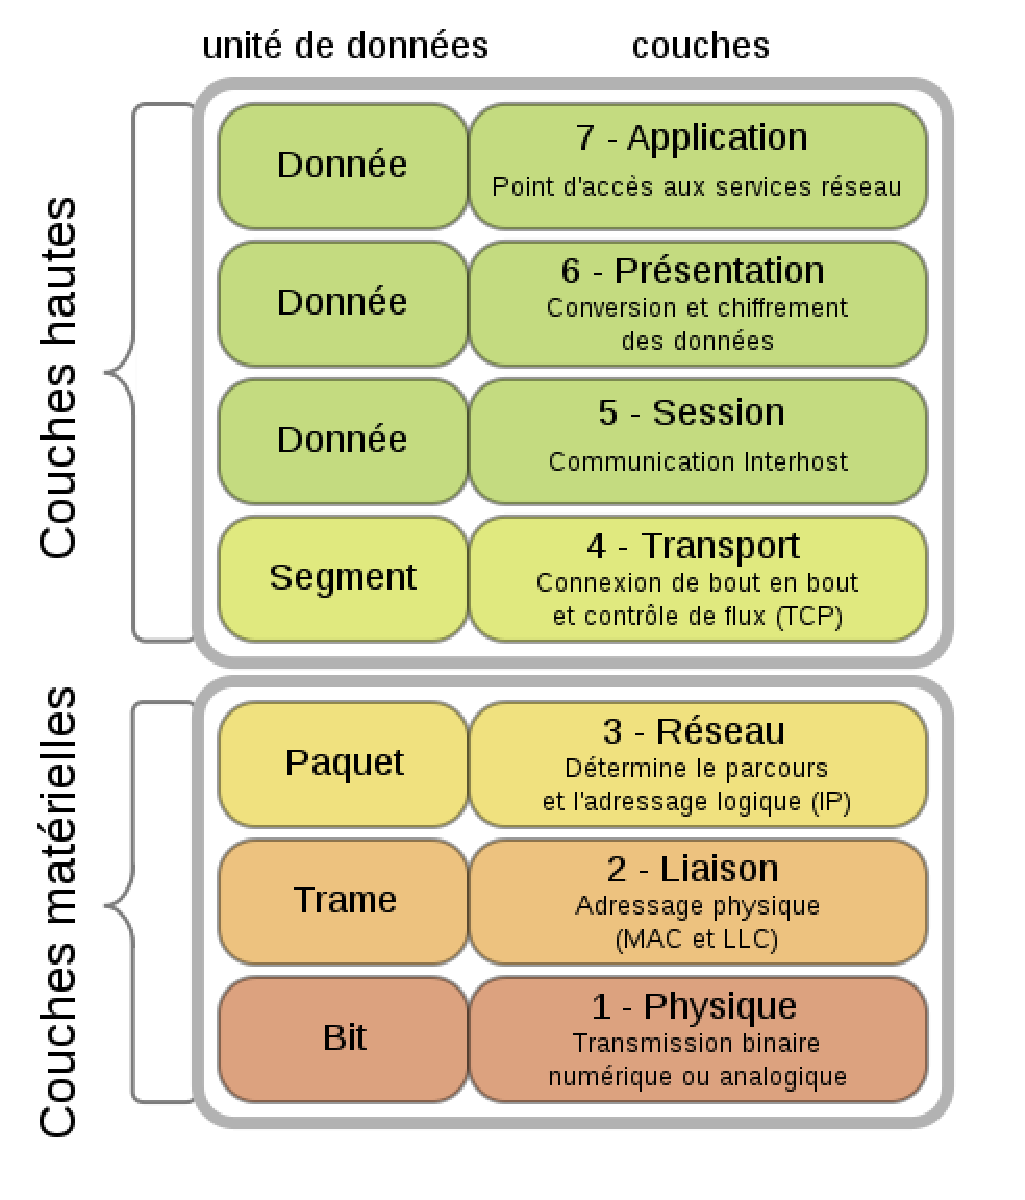
\includegraphics[scale=0.5]{images/osi}
  \caption{Diagramme du modèle OSI}
  \label{fig:osi}
\end{figure}

\section{Spécification X.25}
\subsection{Principe}
Le protocole X.25 ne spécifie pas un réseau à commutation de paquet. Il précise en premier lieu un protocole d'interface d'accès au réseau, c'est-à-dire qu'il définit comment communique un \gls{ETTD},
potentiellement un minitel, avec un nœud du réseau, ce que l'on appelle un \gls{ETCD}\cite{cnam}, voir figure \ref{fig:net}.

\subsection{Normalisation OSI}
Le protocole X.25 intègre les trois couches basses du modèle OSI :

\begin{itemize}
\item couche physique : \textbf{X21} une interface physique et électrique (liaison série) recommandée et publiée par CCITT en 1976 sur la liaison ETTD/ETCD\cite{wikix21}.
\item couche liaison : \textbf{HDLC : LAP-B} assure que les trames arrivent dans l'ordre et sans erreurs, c'est ce qui assure la fiabilité du X.25. La vérification des paquets est faite
par chaque commutateur du réseau X.25, l'ETTD lui ne les fait pas. Il reçoit les paquets dans le bon ordre, il n'a donc pas de traitement supplémentaire à faire. Ce qui fait de l'X.25 un protocole facile
à implémenter sur les machines de faible puissance (processeur et mémoire vive) comme le minitel\cite{wikilapb}.
\item couche réseau : \textbf{X25.3} est le cœur du protocole X.25, il assure la gestion des connexions ainsi que l'adressage\cite{gatoux}. Il détermine aussi comment on envoie des données entre deux ETTD.
\end{itemize}

\subsection{Circuit Virtuel}
Puisque que l'X.25 est un protocole connecté qui fonctionne par commutation de paquets, il utilise un circuit virtuel représenté par une voie logique par connexion. En théorie, X.25 supporte 4096 ($2^{16}$ voir figure \ref{fig:x25}) voies logiques mais dans la pratique, 256 voies logiques sont permises par ETTD.
Un circuit virtuel, une fois établi, permet de considérer la connexion entre deux ETTD comme une liaison directe (abstraction du réseau de transport) de la même manière qu'une liaison téléphonique usuelle\cite{navarro}.

On peut ouvrir deux types de circuits virtuels :
\begin{itemize}
\item \gls{CVP} qui établit de façon permanente, ce qui supprime la phase de connexion, donc un gain de temps. Intéressant si on a un traffic régulier sur la ligne, par contre excessivement coûteux.
\item \gls{CVC} demande quant à lui une phase de connexion. C'est lors de cette phase que seront négociées les options et que l'on attribuera un numéro de voie logique. Pour établir la communication, on utilise le type de paquet \og CALL REQUEST \fg, voir figure~\ref{fig:x25}, dans lequel figureront les adresses destinataire et expéditeur. Ces adresses sont au format défini par la norme X121\cite{navarro}\cite{gateau}.
\end{itemize}

\subsection{Adressage}
X.121 est défini par le CCITT comme : \og Plan de numérotation international pour les réseaux de données publiques \fg.

C'est une norme d'adressage des réseaux. Elle est comparable à l'adressage E.164 (numérotation téléphonique) ou à l'adressage IP. Elle est principalement utilisée comme solution d'adressage par le protocole X.25 pour l'établissement de circuits virtuels commutés. D'autres protocoles, tel que Frame relay, peuvent utiliser X.121\cite{wikix121}.

\begin{figure}[htp]
  \centering
  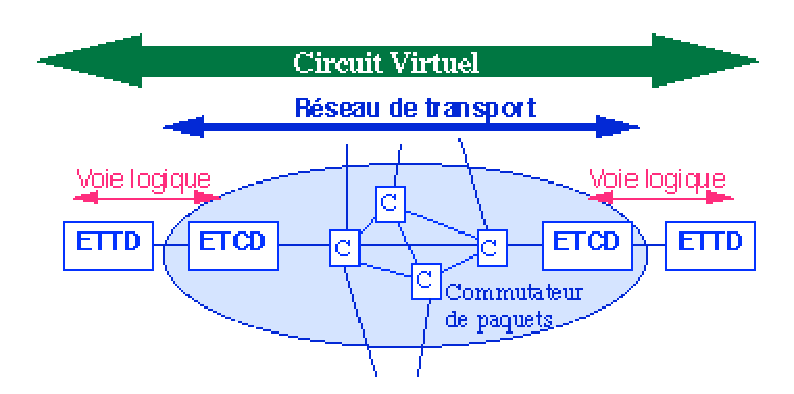
\includegraphics[scale=0.8]{images/network}
  \caption{Réseau X.25}
  \label{fig:net}
\end{figure}

\begin{figure}[htp]
  \centering
  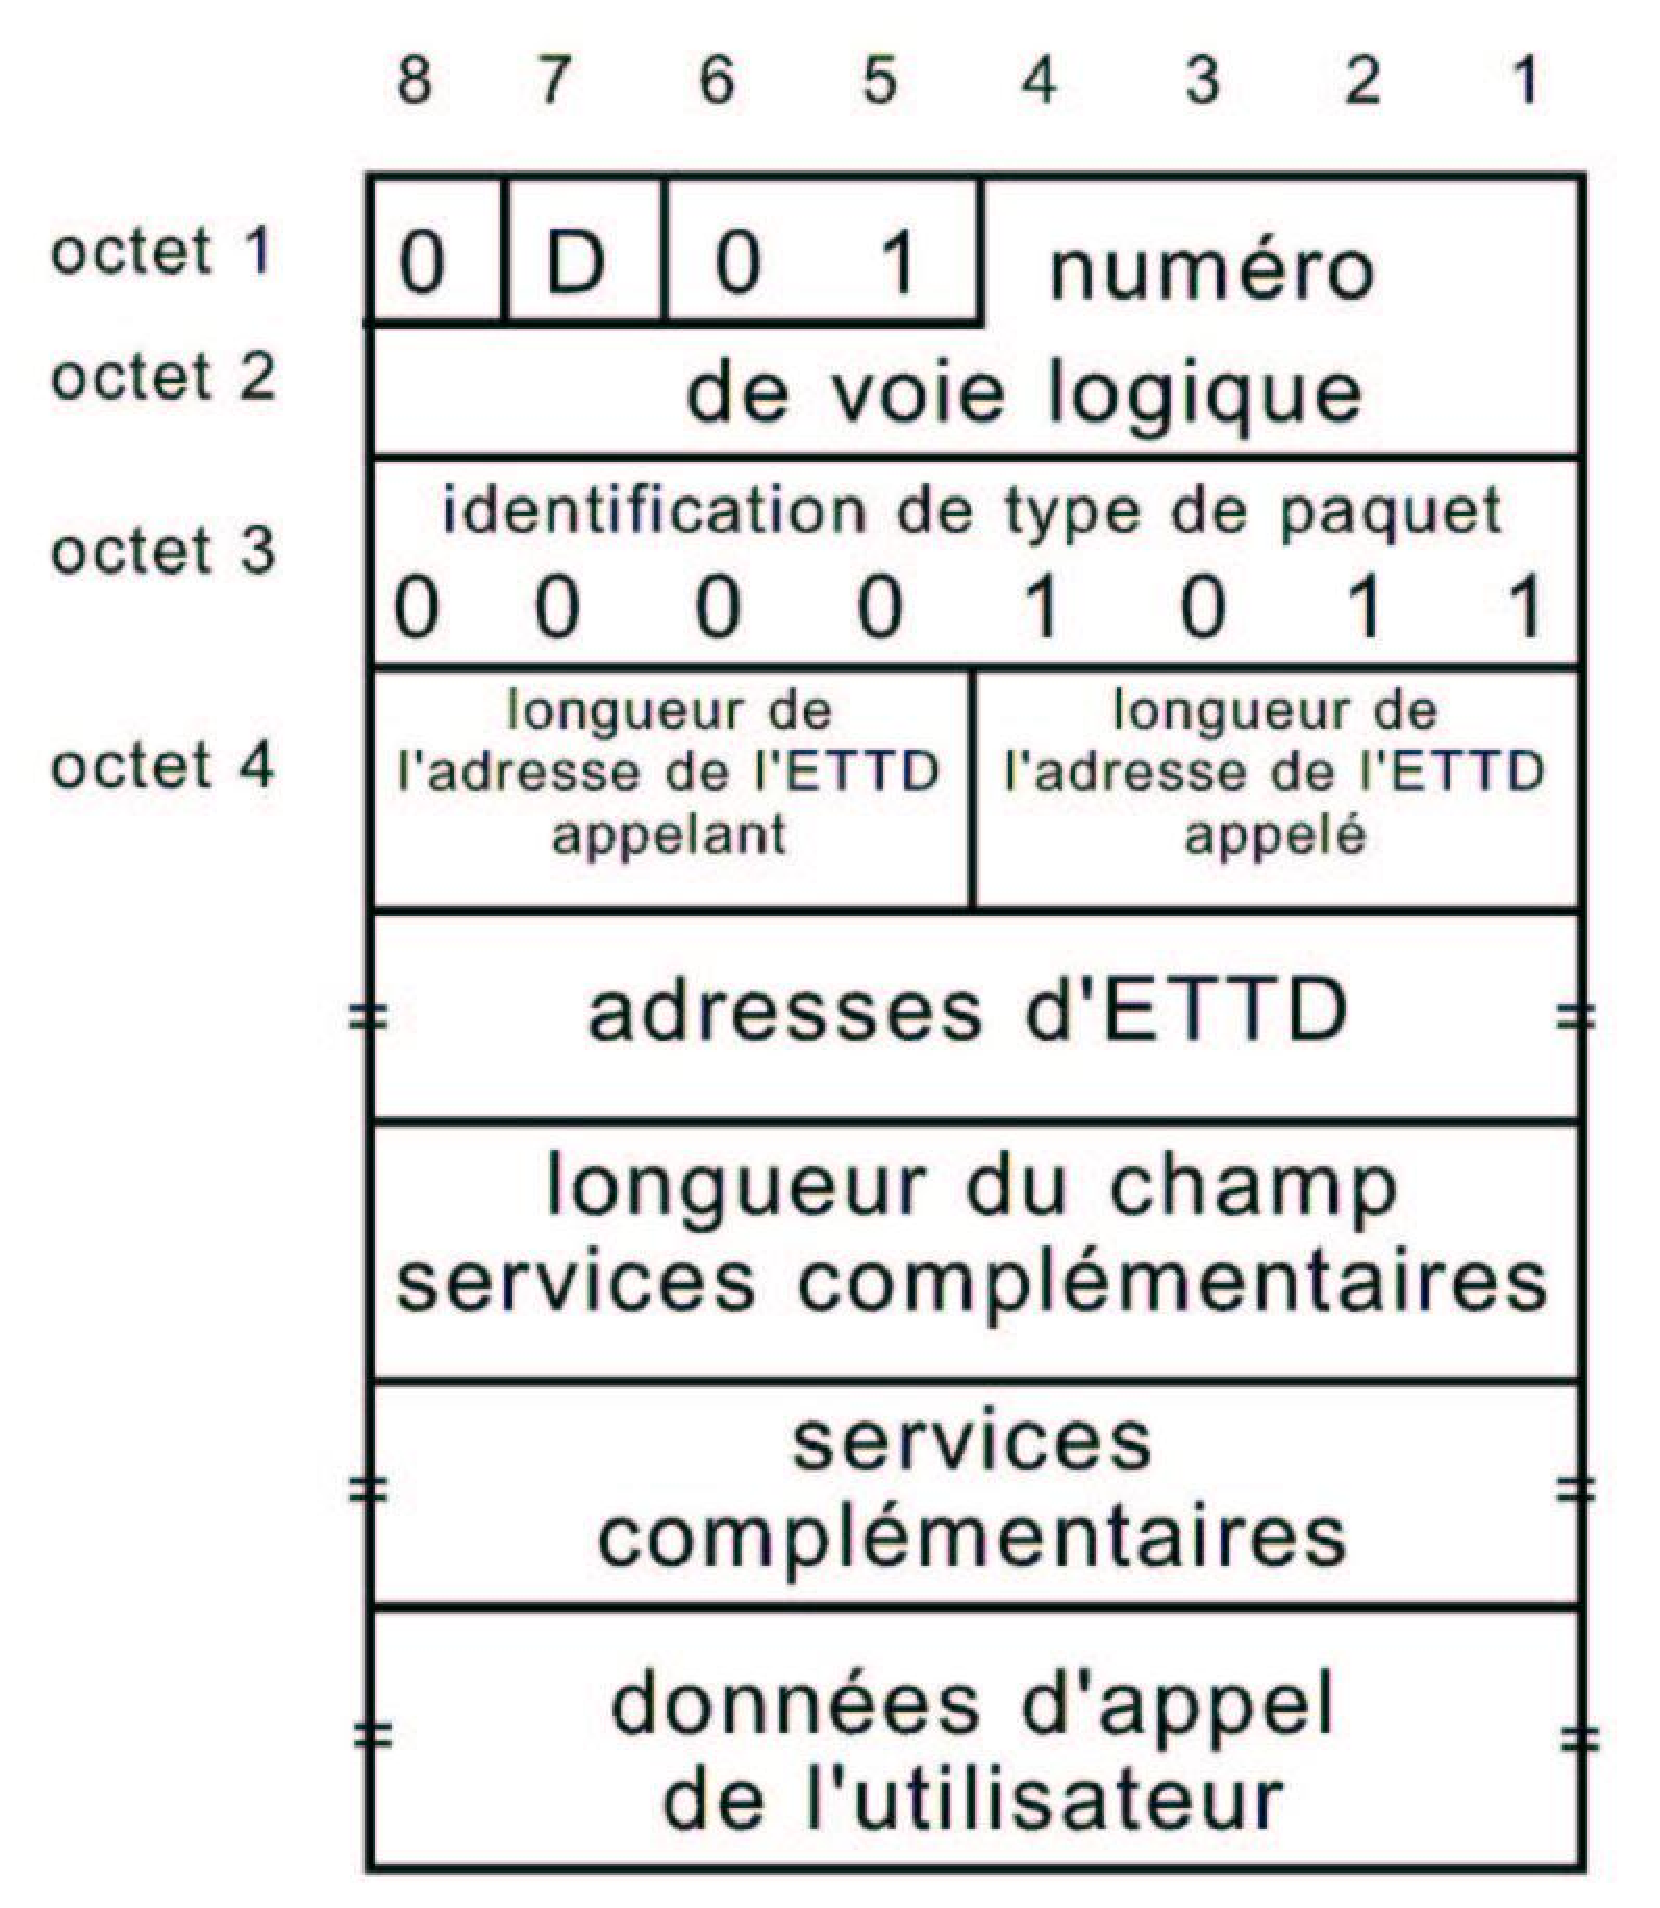
\includegraphics[scale=0.3]{images/x25}
  \caption{Trame X.25 \og CALL REQUEST \fg}
  \label{fig:x25}
\end{figure}

\section{TCP/IP}

À la même époque est développée la suite TCP/IP en 1973 et qui sera adoptée par l'\gls{ARPANET} en 1983. La suite TCP/IP est l'ensemble des protocoles utilisés pour le transfert des données sur Internet. Elle est souvent appelée TCP/IP, d'après le nom de ses deux premiers protocoles : \gls{TCP} et \gls{IP}. Ils ont été inventés par Vinton G. Cerf et Bob Kahn.

Le modèle OSI, qui décompose les différents protocoles en sept couches, peut être utilisé pour décrire la suite de protocoles Internet, bien que les couches du modèle OSI ne correspondent pas toujours avec les habitudes d'Internet puisque qu'Internet est basé sur TCP/IP qui ne comporte que quatre couches, voir figure~\ref{fig:osi-tcp}. Il serait trop long de décrire tous les protocoles de chaque couche du modèle TCP/IP, voici donc une brève description des deux protocoles principaux du modèle TCP/IP\cite{wikitcpip}.

Le protocole IP permet un service d'adressage unique pour l'ensemble des terminaux connectés. Il correspond à la couche Internet (Réseau) du modèle TCP/IP. Il utilise l'adressage IPv4 ou IPv6 en fonction de la version du protocole IP. Il est \og non fiable \fg{} car la fiabilité est assurée par le protocole TCP\cite{wikiip}.

Le protocole TCP est un protocole de transport fiable, en mode connecté. Il correspond à la couche transport du modèle TCP/IP. La fiabilité et la validité des paquets sont garanties, à la différence que le protocole ne respecte pas l'ordre de séquencement des paquets, ce qui est tout à fait normal puisqu'il utilise des datagrammes. C'est pour cette raison qu'une connexion TCP est évidemment virtuel, représentée par un port. Le protocole TCP peut ouvrir un maximum de $2^{16}$ ports, soit 65536 connexions théoriques. La vérification des paquets est réalisée par les terminaux émetteur et récepteur des paquets, surtout par le récepteur qui doit garder en mémoire tous les paquets pour compléter le message final\cite{wikitcp}.

\begin{figure}[htp]
  \centering
  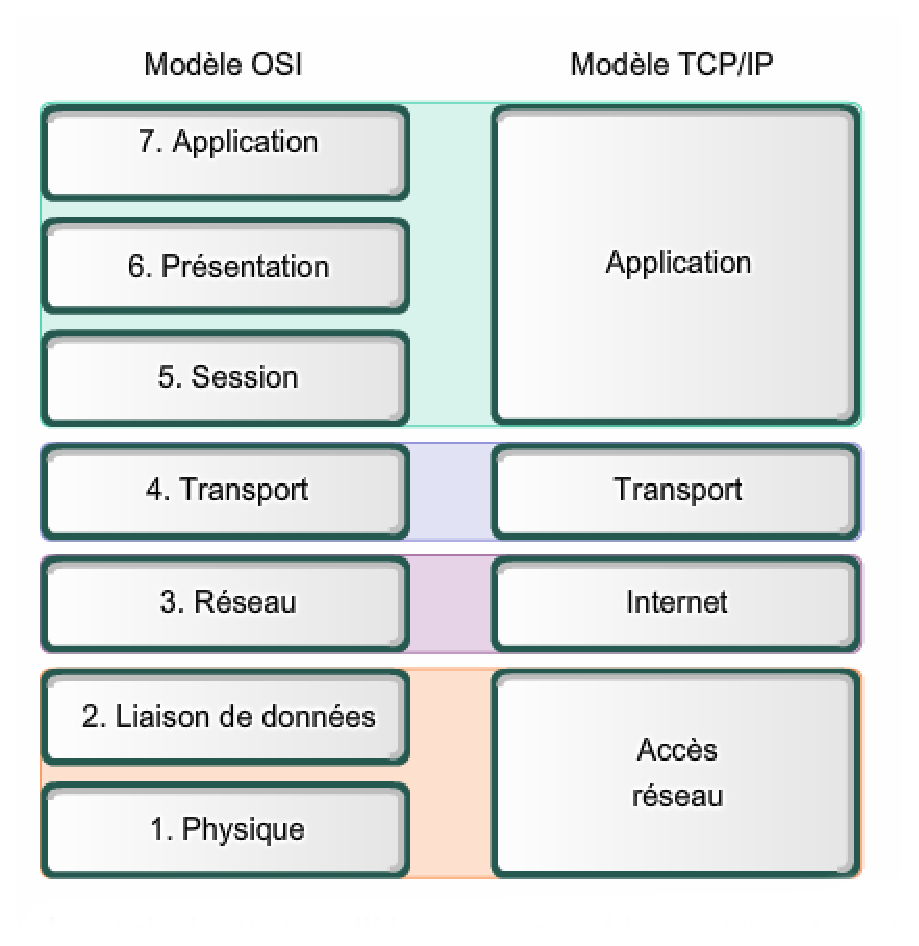
\includegraphics[scale=0.5]{images/osi-tcp-ip}
  \caption{Comparaison modèle OSI et TCP/IP}
  \label{fig:osi-tcp}
\end{figure}

\section{Conclusion}

Malheureusement la fiabilité de l'X.25, c'est-à-dire l'ordre de séquencement des paquets, si cher aux yeux des PTTs, a un prix.
Chaque nœud d'échange de paquets (Packet-Switching Exchanger) doit vérifier la validité du paquet qui
transite par lui, ce qui limite et ralenti le nombre de connexions par échangeur. Tout le contraire du TCP qui contrôle les paquets à la réception par le destinataire.
L'économie de traitement réalisée par l'X.25 pour les ETTDs devient problèmatique par la suite surtout qu'elle n'a plus lieu d'être avec les avancées dans les composants informatiques.
De plus, le protocole X.25 est limité à 4096 connexions alors que le protocole TCP peut en ouvrir théoriquement 65536. Les nœuds d'X.25 sont donc inférieurs en capacité et en vitesse face à la suite TCP/IP.
Outre ces différences de vitesse, le protocole X.25 pose des problèmes d'intéropérabilité et de monopole. Les différents constructeurs de l'époque (IBM, Digital), fort de leur monopole,
ont fait tout leur possible pour rendre leurs matériels incompatibles entre eux pour des raisons de concurrence, ce qui complique le travail des entreprises pour
communiquer entre-elles et leurs différents interlocuteurs\cite{gatoux}. Le monopole d'exploitation de Transpac a forcé les opérateurs concurrents à s'orienter sur TCP/IP.
Le X25 souffrait donc d'un problème d'ouverture et d'unification, ce qui n'est pas le cas avec l'encapsulation du TCP/IP,
qui peut s'adapter à n'importe quelle application à travers son réseau. Le dernier commutateur X.25 du réseau Orange est éteint le 12 mai 2017\cite{killme}.

Pour méditer... Selon Maurice Allègre, délégué à l'informatique du Plan Calcul :

\og Louis Pouzin, polytechnicien et chercheur de très grand talent, (est à l'époque) venu proposer un projet de réseau maillé d'ordinateurs basé sur quelque chose de totalement nouveau : la commutation de paquets. « Très vite, les recherches ont connu un plein succès, au point que j'ai déployé de grands efforts pour faire adopter le projet par la direction générale des télécommunications comme base pour leur futur réseau de transmissions de données », dit M. Allègre dans un courrier. « Je me suis malheureusement heurté à un mur. (Les ingénieurs des télécoms préfèrent pousser le développement industriel du Minitel. ) Nous aurions pu être parmi les pionniers du monde Internet (...)», conclut le courrier de l'ancien haut fonctionnaire. Nous n'en sommes que des utilisateurs, fort distants des lieux où s'élabore l'avenir. \fg\cite{wikipouzin}

% ~=~=~=~=~=~=~=~=~=~=~=~=~
% Le premier vol d'Ariane 5
% ~=~=~=~=~=~=~=~=~=~=~=~=~

\chapter{Le premier vol d'Ariane 5}

\section{Introduction}

Le 4 juin 1996, le premier vol d'Ariane 5 a échoué. Après 37 secondes de vol, la fusée explose à 4000 mètres d'altitude 
détruisant par le même occasion sa charge utile constituée de 4 satellites, d'une valeur total de 370 millions de dollars.
À la suite de l'incident, le CNES a demandé une enquête afin de déterminer les causes de l'incident.

\section{Le déroulement du crash}

Environ 30 secondes après le décollage, la centrale à inertie de secours est devenu inopérante à cause d'une variable relative à l'accélération horizontale de l'appareil. L'incident s'est passé lors d'une conversion    
d'un nombre à virgule codé sur 64 bits vers un entier signé codé sur 16 bits. Le nombre à virgule à convertir avait une valeur trop grande pour être converti en entier sur 16 bits. De plus il avait été décidé de ne pas mettre en place de mesure de protection contre cette erreur lors de son écriture pour Ariane 4 car la variable ayant dépassée est dépendante de la vitesse de l'appareil. Pour Ariane 4 cela ne posait aucun problème car la vitesse maximale de la fusée était trop faible pour générer ce dépassement de mémoire. Cependant, Ariane 5 est une fusée plus puissante qu'Ariane 4 et sa vitesse à donc dépassé la limite qui garantissait qu'aucune erreur de ce type ne se produise \cite{ariane}.

Environ 0.05 secondes plus tard la centrale à inertie active a subi le même problème mais étant donné que le système de secours n'était déjà plus opérationnel, plus aucune information concernant l'altitude et le guidage de la fusée n'était disponible.   

L'ordinateur principal a alors interprété les données diagnostiques de la centrale à inertie comme des données de vol et a entrepris une correction de trajectoire d'une déviation qui, au final, n'a jamais eu lieu.
  
Cette nouvelle trajectoire a entrainé un changement brutal d'altitude qui a lui même causé la désintégration du lanceur de la fusée. Cette désintégration a alors  enclenché l'auto-destruction de la fusée à une altitude de 4000 mètres.

De plus le \gls{CNES} a demandé de ne pas faire de simulations de vol pour le système de navigation pour faire des économies car celui-ci avait été récupéré d'Ariane 4 et était considéré comme fiable.

Enfin, le même code a été placé dans les deux centrales à inertie, ce qui a inévitablement permis au bug de se produire dans les deux centrales. 

\section{Les solutions possibles}
Une des premières causes de cet échec est tout d'abord le faible budget alloué pour le développement d'Ariane 5.
Dès le début du projet le CNES et L'\gls{ESA} ont dû s'arranger pour réduire le plus possible le coût de réalisation de la fusée. C'est dans ce que contexte qu'ont été décidés les choix de réutiliser le code d'Ariane 4, celui de placer ce même code dans les deux centrales à inertie ainsi que le choix de ne pas réaliser de simulation de vol, tout cela dans le but de limiter le coût de production de cette fusée.

Pour ce problème de budget, on ne peut présenter de réelles solutions. Le seul moyen d'éviter ces choix aurait été d'avoir un budget plus important en premier lieu.

En revanche, si l'on aborde les solutions qui aurait pu détecter et empêcher le dépassement mémoire en lui même alors on peut en voir plusieurs. Premièrement, rappeler l'importance d'utiliser des programmes développés de manière indépendante pour un ordinateur ainsi que celui de secours. Cela permet d'éviter qu'une même erreur se produise sur les deux ordinateurs comme dans le cas d'Ariane 5. Le problème avec cette technique, c'est qu'elle ne permet pas de garantir que notre programme ne génère aucun bug et qu'il a bien le comportement souhaité et spécifié. Donc pour éviter ce dépassement mémoire, on peut aussi utiliser diverses méthodes prouvant que notre programme a le comportement souhaité peu importe la situation. Ces diverses techniques sont regroupées sous le nom de méthodes formelles. 
\section{Les méthodes formelles }
\subsection{Présentation}
Les méthodes formelles sont des méthodes qui utilisent les mathématiques afin de démontrer qu'un système informatique respecte parfaitement ses spécifications. Les méthodes formelles sont à l'heure actuelle surtout utilisées sur les systèmes dits critiques.

Un système critique est un système informatique qui, en cas de dysfonctionnement, peut causer des morts ou des blessés, des coût matériels élevés ou de graves conséquences pour l'environnement. Par exemple dans le domaine du transport, de la santé ou même de l'énergie.

La plupart des méthodes formelles ont été théorisées dans les années 80 mais n'ont pu être appliquées que bien plus tard à cause des limitations techniques des ordinateurs de l'époque. 

De plus ces méthodes, même quand elles étaient techniquement appliquables, ont mis du temps à s'imposer dans les entreprises car les ingénieurs de l'époque ne trouvaient pas d'intérêt à utiliser de telles méthodes. Cependant, durant les années 2000, les méthodes formelles sont de plus en plus utilisées dans les entreprises car de nouveaux employés formés à ces méthodes font leur apparition dans les entreprises. De plus, l'\gls{EAL},un système d'évaluation de la sécurité d'un système informatique, a recours aux méthodes formelles afin de réaliser son évaluation, incitant les développeurs à eux même utiliser les méthodes formelles lors de la création de leur solution \cite{griffault}.    

Il existe plusieurs méthodes intervenant à divers moments du cycle de vie du développement. Elles seront présentés dans les prochaines sections.   
\subsection{Vérification de modèles}
La vérification par modèle est la méthode formelle la plus utilisée à l'heure actuelle au sein de l'industrie \cite{griffault}. Elle permet de vérifier si le modèle d'un système respecte diverses propriétés. Si la propriété n'est pas vérifiée, on renvoie un contre-exemple qui l'invalide. 

Un modèle est un graphe dont chaque sommet représente un état du système.

Il existe deux types de propriété à vérifier.

En premier on peut citer les propriétés de sécurité. Par exemple, dans le cas d'un ascenseur, cela serait la propriété "Un ascenseur doit toujours voyager les portes fermées".

Puis il y a les propriétés de vivacité. Pour reprendre le cas de l'ascenseur, on pourrait avoir "L'ascenseur ramasse les utilisateurs qui l'appelle".   

Un des grands désavantages de cette méthode est que la taille du modèle devient très rapidement extrêmement grande et impossible à utiliser en fonction du système que l'on veut mettre en place.
   
Cependant, la vérification de modèles est une méthode particulièrement efficace lorsqu'elle est utilisée pour vérifier des protocoles réseaux. La vérification de modèles a par exemple été utilisée pour trouver FREAK, une faille des protocoles SSL/TLS. Grâce à cette méthode, des équipes conjointes de l'INRIA et de Microsoft ont ainsi prouvé que les protocoles faisaient bien plus que ce qui était spécifié et que cela était à l'avantage de potentiels attaquants \cite{goubault}.    

\subsection{Génération de tests}
La génération de tests fonctionne de la même manière que la vérification de modèle. On créé un modèle et au lieu de chercher à vérifier une propriété, on définit toutes les actions à faire pour qu'une propriété soit vrai. Cette suite d'actions nous donne le test à réaliser pour vérifier notre propriété \cite{griffault}.

\subsection{Démonstration de théorèmes}
Le but initial ici est de faire en sorte que des logiciels puissent réaliser une démonstration d'une proposition de façon totalement autonome. Cependant les problèmes abordés sont souvent trop profonds pour qu'un logiciel puisse réaliser cela tout seul. En conséquence, il existe des logiciels qui permettent à une personne de résoudre plus facilement des problèmes. Ces logiciels s'appellent des assistants de preuve. 

Les assistants de preuve sont assez pratiques pour démontrer qu'un algorithme réalise bien ce pourquoi on l'a crée. En revanche, cette méthode a le désavantage de demander une personne hautement spécialisée dans ce domaine pour pouvoir apporter un réel plus à contrario des méthodes déjà citées et à venir \cite{griffault}.

Un des plus grand succès des assistants de preuve a sûrement été la réalisation d'une preuve formelle du théorème des quatre couleurs. Ce théorème stipule qu'il est possible de colorier une carte avec quatre couleurs uniquement et sans qu'une même couleur se trouve sur deux régions adjacentes de cette carte. Ce théorème à donc été prouvé en 2004 à l'aide de l'assistant de preuve Coq, développé par l'INRIA \cite{delahaye}.     

\subsection{Raffinement}

Le raffinement est une méthode qui permet de transformer des spécifications, donc un niveau assez abstrait, à une implémentation par un système d'itérations tout en garantissant à chaque étape de ce raffinement la conservation des propriétés du système. De plus, chaque itération du raffinement doit être prouvée par la méthode de démonstration de théorème.

Le raffinement est utilisé dans la méthode B, une méthode permettant de spécifier un logiciel en langage B et d'y appliquer un raffinement jusqu'à obtenir une implémentation finale qui peut ensuite être traduite en C ou en Ada. Cette méthode a notamment permis de réaliser le projet météor, à savoir l'automatisation totale de la ligne 14 du métro parisien. Cette méthode a également permis de certifier le système de cette ligne de métro sans avoir recours à des vérifications a posteriori \cite{griffault}.      
\subsection{Langages dédiés}
Un langage dédié est un langage offrant des primitives et des abstractions qui permettent de travailler plus efficacement dans un domaine particulier. Le haut niveau d'abstraction permet aux professionnels du domaine concerné de ne se concentrer que sur les problèmes de son domaine et non les problèmes de plus bas niveau, limitant ainsi les erreurs possibles et rendant plus facile la validation d'une solution par ces même experts \cite{Deuklvi}. On peut ici citer Bison et Lex permettant de travailler respectivement sur les analyseurs syntaxiques et lexicaux.
\subsection{Interprétation abstraite}
Avec l'interprétation abstraite, on part du programme et on tente d'approximer sa sémantique. On réduit donc un problème complexe, notre programme, en un modèle abstrait. Avec cela, un analyseur peut comparer l'approximation du comportement du programme avec les spécifications de base, et si un problème a lieu, l'analyseur peut donner des pistes afin de corriger l'erreur trouvée.

Cette méthode permet de raisonner sur des programmes de grande taille en imposant un niveau d'approximation assez élevé. Le problème, c'est que ce niveau d'approximation ne nous permet alors de verifier que des propriétés très basiques portant très souvent sur l'absence d'erreurs d'exécution \cite{cousot}.    
\subsection{Analyse de code binaire}

L'analyse de code binaire est une méthode très récente et encore en pleine évolution. C'est une méthode permettant de désassembler un exécutable afin de vérifier si certaines propriétés d'un programme sont valides même sans avoir le code source. 

C'est une méthode qui peut être utilisée sur des systèmes auxquels on peut rajouter des modules afin de vérifier que le module ne modifie pas les propriétés de tout le système et que celui-ci reste bien assigné à son rôle \cite{griffault}.
\subsection{Limites}

Il faut tout de même apporter un peu de nuances à tout cela. Les méthodes formelles ne sont pas infaillibles. Elle ne garantissent pas impérativement qu'un programme soit sans bug.

Tout d'abord, il faut que les modèles créés ait un sens, à force de complexifier un modèle pour respecter les propriétés les plus compliquées, on peut finir par ne plus pouvoir faire des actions qui étaient pourtant simple dans le modèle de base. 

Pour les démonstrations de théorèmes, pour qu'une démonstration soit valide, il faut que le logiciel d'aide à la preuve utilisé soit lui aussi prouvé au préalable, ce qui est très dur à faire.

Et pour finir, il faut aussi se rappeler que le fait qu'un algorithme fasse réellement ce qu'on lui demande est bien souvent un problème indécidable \cite{griffault}.

Les méthodes formelles sont donc de formidables outils à condition de ne pas tout miser sur elles lors du développement afin d'obtenir un programme qui fonctionne comme souhaité.

\printglossaries
\printbibliography

\end{document}
